% Options for packages loaded elsewhere
\PassOptionsToPackage{unicode}{hyperref}
\PassOptionsToPackage{hyphens}{url}
%
\documentclass[
  12pt,
]{article}
\usepackage{lmodern}
\usepackage{amssymb,amsmath}
\usepackage{ifxetex,ifluatex}
\ifnum 0\ifxetex 1\fi\ifluatex 1\fi=0 % if pdftex
  \usepackage[T1]{fontenc}
  \usepackage[utf8]{inputenc}
  \usepackage{textcomp} % provide euro and other symbols
\else % if luatex or xetex
  \usepackage{unicode-math}
  \defaultfontfeatures{Scale=MatchLowercase}
  \defaultfontfeatures[\rmfamily]{Ligatures=TeX,Scale=1}
\fi
% Use upquote if available, for straight quotes in verbatim environments
\IfFileExists{upquote.sty}{\usepackage{upquote}}{}
\IfFileExists{microtype.sty}{% use microtype if available
  \usepackage[]{microtype}
  \UseMicrotypeSet[protrusion]{basicmath} % disable protrusion for tt fonts
}{}
\makeatletter
\@ifundefined{KOMAClassName}{% if non-KOMA class
  \IfFileExists{parskip.sty}{%
    \usepackage{parskip}
  }{% else
    \setlength{\parindent}{0pt}
    \setlength{\parskip}{6pt plus 2pt minus 1pt}}
}{% if KOMA class
  \KOMAoptions{parskip=half}}
\makeatother
\usepackage{xcolor}
\IfFileExists{xurl.sty}{\usepackage{xurl}}{} % add URL line breaks if available
\IfFileExists{bookmark.sty}{\usepackage{bookmark}}{\usepackage{hyperref}}
\hypersetup{
  pdftitle={Voting in a Pandemic: COVID-19 and Primary Turnout in Milwaukee, Wisconsin},
  pdfauthor={Kevin Morris; Peter Miller},
  hidelinks,
  pdfcreator={LaTeX via pandoc}}
\urlstyle{same} % disable monospaced font for URLs
\usepackage[margin=1in]{geometry}
\usepackage{longtable,booktabs}
% Correct order of tables after \paragraph or \subparagraph
\usepackage{etoolbox}
\makeatletter
\patchcmd\longtable{\par}{\if@noskipsec\mbox{}\fi\par}{}{}
\makeatother
% Allow footnotes in longtable head/foot
\IfFileExists{footnotehyper.sty}{\usepackage{footnotehyper}}{\usepackage{footnote}}
\makesavenoteenv{longtable}
\usepackage{graphicx}
\makeatletter
\def\maxwidth{\ifdim\Gin@nat@width>\linewidth\linewidth\else\Gin@nat@width\fi}
\def\maxheight{\ifdim\Gin@nat@height>\textheight\textheight\else\Gin@nat@height\fi}
\makeatother
% Scale images if necessary, so that they will not overflow the page
% margins by default, and it is still possible to overwrite the defaults
% using explicit options in \includegraphics[width, height, ...]{}
\setkeys{Gin}{width=\maxwidth,height=\maxheight,keepaspectratio}
% Set default figure placement to htbp
\makeatletter
\def\fps@figure{htbp}
\makeatother
\setlength{\emergencystretch}{3em} % prevent overfull lines
\providecommand{\tightlist}{%
  \setlength{\itemsep}{0pt}\setlength{\parskip}{0pt}}
\setcounter{secnumdepth}{5}
\usepackage{rotating}
\usepackage{setspace}
\usepackage{booktabs}
\usepackage{longtable}
\usepackage{array}
\usepackage{multirow}
\usepackage{wrapfig}
\usepackage{float}
\usepackage{colortbl}
\usepackage{pdflscape}
\usepackage{tabu}
\usepackage{threeparttable}
\usepackage{threeparttablex}
\usepackage[normalem]{ulem}
\usepackage{makecell}
\usepackage{xcolor}
\newlength{\cslhangindent}
\setlength{\cslhangindent}{1.5em}
\newenvironment{cslreferences}%
  {\setlength{\parindent}{0pt}%
  \everypar{\setlength{\hangindent}{\cslhangindent}}\ignorespaces}%
  {\par}

\title{Voting in a Pandemic: COVID-19 and Primary Turnout in Milwaukee, Wisconsin}
\author{Kevin Morris\footnote{Researcher, Brennan Center for Justice at NYU School of Law, 120 Broadway Ste 1750, New York, NY 10271 (\href{mailto:kevin.morris@nyu.edu}{\nolinkurl{kevin.morris@nyu.edu}})} \and Peter Miller\footnote{Researcher, Brennan Center for Justice at NYU School of Law, 120 Broadway Ste 1750, New York, NY 10271 (\href{mailto:peter.miller@nyu.edu}{\nolinkurl{peter.miller@nyu.edu}})}}
\date{December 06, 2020}

\begin{document}
\maketitle
\begin{abstract}
We report the first study of the effect of the novel coronavirus SARS-CoV-2 (COVID-19) on polling place consolidation and voting behavior. We draw upon individual-level observations from Milwaukee matched to similar observations in the surrounding municipalities to assess whether fewer polling places in the April presidential primary election decreased turnout in the city. We find polling place consolidation reduced overall turnout by about \textbf{8.9} points and reduced turnout among the Black population in the city by about \textbf{10.4} points. We conclude on the basis of these data that conversion to widespread absentee voting in the general election may have resulted in disenfranchisement, particularly among racial minorities.
\end{abstract}

\pagenumbering{gobble}
\pagebreak

\pagenumbering{arabic}
\doublespacing

The Wisconsin presidential primary election provides a valuable means to assess how the novel coronavirus SARS-CoV-2 (COVID-19) has altered voting behavior in a natural experiment. The weeks leading up to the presidential primary election on April 7 were tumultuous. Democratic Governor Tony Evers declared a state of emergency on March 12 when there were 8 confirmed COVID-19 cases.\footnote{See \url{https://www.dhs.wisconsin.gov/covid-19/cases.htm}.} On March 17, Evers issued a ban on all gatherings of more than 10 people.\footnote{See \url{https://evers.wi.gov/Documents/COVID19/UPDATEDOrder10People.pdf}.} On March 27, Evers called for every voter in the state to be sent an absentee ballot (Wise \protect\hyperlink{ref-Wise2020}{2020}). The Republican-controlled legislature refused this proposal. The weekend before the election, Evers called an emergency session of the legislature hoping to postpone the date of the election. This effort, too, was rebuffed. As a last resort, Evers issued an executive order on April 6 to delay the primary election until the ninth of June\footnote{See \url{https://bit.ly/3fJTqZT}.} which was overturned by the state supreme court.\footnote{See \url{https://wapo.st/2Cg79sK}.} The U.S. Supreme Court also ruled absentee ballots would be invalid if the ballot was not hand-delivered by April 7 or postmarked by election day and received by April 13.\footnote{See \url{https://www.supremecourt.gov/opinions/19pdf/19a1016_o759.pdf}.}

These maneuvers occurred against the backdrop of overstretched electoral resources following from the increasing severity of the COVID-19 pandemic. The \emph{Milwaukee Journal Sentinel} observed the state was short some 7 thousand poll workers on March 31 (Marley and Beck \protect\hyperlink{ref-Marley2020}{2020}), a shortage which led to widespread polling place consolidation. The reduction in polling places was acute in Milwaukee. Five polling places remained open, compared with 182 in November of 2016.\footnote{See \url{https://elections.wi.gov/elections-voting/2016/fall} and \url{https://elections.wi.gov/node/6524}.} Even as polling places were consolidated, a surge in absentee voting occurred. Statewide, more than 964 thousand ballots were cast by mail in the April primary, compared with 171 thousand in the 2016 presidential primary.\footnote{See \url{https://elections.wi.gov/sites/elections.wi.gov/files/2020-05/April\%202020\%20Absentee\%20Voting\%20Report.pdf}.} Nonetheless, there is evidence for ``leaked'' absentee ballots that were excluded from the set of counted ballots (Stewart \protect\hyperlink{ref-Stewart2010}{2010}): only 84.8 percent of mail ballots delivered to voters were ultimately counted. Past research indicates that, under normal circumstances, polling place consolidation leads to lower turnout (e.g.~Brady and Mcnulty \protect\hyperlink{ref-Brady2011}{2011}; McNulty, Dowling, and Ariotti \protect\hyperlink{ref-McNulty2009}{2009}). \textbf{The circumstances in Milwaukee, in contrast to these earlier studies of polling place consolidation, are novel in that consolidation here was a consequence of a natural disaster rather than of an administrative decision to reallocate polling places.}

This study asks two key questions. First, we investigate whether polling place consolidation measurably decreased overall turnout in the context of a primary election with widespread access to vote-by-mail options. Just 16.1 percent of registered voters in the City of Milwaukee voted in the April primary, while the overall turnout rate in the rest of Milwaukee County and surrounding Waukesha, Washington, and Ozaukee Counties was 42.2 percent. Second, we aim to measure whether COVID-19, which was more widespread in the City of Milwaukee, depressed turnout through other mechanisms. The opportunity cost literature indicates that household shocks like family emergencies can make it less likely that voters invest the time and resources needed to learn where their polling places are and who is on the ballot.

\hypertarget{prior-literature}{%
\subsubsection*{Prior Literature}\label{prior-literature}}
\addcontentsline{toc}{subsubsection}{Prior Literature}

\textbf{Election administration in the United States is defined by two values: decentralized authority and oversight by partisan, elected officials (Gerken \protect\hyperlink{ref-Gerken2007}{2007}). Election administration in Wisconsin is an extreme version of the first value. While county officials tend to be the front line administrators for elections, in Wisconsin this task is a duty of officials in each municipality, of which there are 1,851 (Huefner et al. \protect\hyperlink{ref-Huefner2007}{2007}, 111--36). The population disparity between Milwaukee on the one hand and rural parts of the state is vast and raises questions of equal administrative capacity (Kimball and Baybeck \protect\hyperlink{ref-Kimball2013}{2013}) when it comes to questions like the placement and staffing of polling places in an election (Mickle \protect\hyperlink{ref-Mickle2020}{2020}).}

Disrupting one's routine with regard to voting -- whether by relocating or reducing the number of polling places -- reduces turnout by imposing new search and transportation costs on voters (Brady and Mcnulty \protect\hyperlink{ref-Brady2011}{2011}). A moved polling place reduced the likelihood of voting by about 5.5 points in a 2001 local election (Haspel and Knotts \protect\hyperlink{ref-Haspel2005}{2005}). Consolidation between 2000 and 2008 reduced county-level turnout by about nine-tenths of a point (Kropf and Kimball \protect\hyperlink{ref-Kropf2012}{2012}, 68). Increasing the distance to polls in California in 2003 reduced the likelihood of voting in person by between 2 and 4 points. Absentee voting is more likely as the distance to the polls increases, but (at least in past elections) this effect is not large enough to offset the decrease from consolidation itself (Brady and Mcnulty \protect\hyperlink{ref-Brady2011}{2011}). Consolidating polling places in a New York State local election reduced turnout by an average of 7 points (McNulty, Dowling, and Ariotti \protect\hyperlink{ref-McNulty2009}{2009}). A recent study of nine municipalities in Massachusetts and Minnesota found increasing the distance to the polls by about 0.25 miles reduces turnout by between 2 and 5 points, and that this effect is more pronounced among ``high-minority, low-income, and low-car-availability areas'' in the context of a non-presidential election (Cantoni \protect\hyperlink{ref-Cantoni2020}{2020}, 88).

The effect of distance to the polling place on voting is nonlinear (Dyck and Gimpel \protect\hyperlink{ref-Dyck2005}{2005}, 541--42; Gimpel and Schuknecht \protect\hyperlink{ref-Gimpel2003}{2003}, 481--84). Dyck and Gimpel (\protect\hyperlink{ref-Dyck2005}{2005}) deploy observations ranging from .1 to 65 miles from the polling place. They report being one standard deviation from the polls (about 1.75 miles) reduces the likelihood of voting at the polls by 2.3 points, but makes absentee voting more likely by 0.9 points. A study of three counties in Maryland in the 2000 election finds moving 1 mile \emph{closer} to the polls makes voting \emph{more} likely by 0.45 points, while observing generally ``{[}t{]}urnout is highest when distances to the polling place are very short, and when they are excessively long, but lower in the middling ranges of distance'' (Gimpel and Schuknecht \protect\hyperlink{ref-Gimpel2003}{2003}, 481).

\textbf{Vote centers are an alternative convenience voting reform that could be well-suited to counteract the depressive turnout effects of polling place consolidation. Vote centers are distinguished from polling places in two ways: they are open to all voters in an area (like a county or group of precincts) and are centralized (Stein and Vonnahme \protect\hyperlink{ref-Stein2008}{2008}, 490--91). Vote centers increase turnout among infrequent voters and in low-turnout elections (Stein and Vonnahme \protect\hyperlink{ref-Stein2008}{2008}, \protect\hyperlink{ref-Stein2012}{2012}; but see Cortina and Rottinghaus \protect\hyperlink{ref-Cortina2019}{2019}). That being said, this reform was not adopted in the April primary in Wisconsin. Election officials instead maintained the precinct-based assignment for voters instead of opening each polling place to any registered voter in the county.}

The literature discussed above, however, examines the effect of polling place consolidation under more normal circumstances. It is unclear whether that is the case in elections held during a pandemic. Indeed, with more than 97 percent of polling places in Milwaukee City closed, the primary contest may be better understood as an example of conducting elections entirely by mail, as is the case in some western states. That reform increases turnout in Washington (Henrickson and Johnson \protect\hyperlink{ref-Henrickson2019}{2019}; Gerber, Huber, and Hill \protect\hyperlink{ref-Gerber2013}{2013}), decreases turnout in California (Elul, Freeder, and Grumbach \protect\hyperlink{ref-Elul2017}{2017}; Bergman and Yates \protect\hyperlink{ref-Bergman2011}{2011}; Kousser and Mullin \protect\hyperlink{ref-Kousser2007}{2007}), and has no significant effect in Oregon (Gronke and Miller \protect\hyperlink{ref-Gronke2012}{2012}). That the same reform has disparate effects where it has been adopted is one reason scholars are left unsatisfyingly answering the question about turnout effects of convenience voting reforms with both ``\,`no' and `yes'\,'' (Bergman \protect\hyperlink{ref-Bergman2015}{2015}). Of course, these shifts to vote-by-mail were long-term, planned policy changes that were accompanied by voter education programs. It seems likely that a last-minute decision to conduct the election this way would be less successful at mitigating any depressive effects.

This literature provides the framing for Hypothesis A: By both increasing the distance voters had to travel to arrive at their polling places and requiring that they learn the location of the new polling place, we expect that turnout was lower in the City of Milwaukee due to the polling place consolidation.

\textbf{Of course, the City of Milwaukee was also home to a worse COVID-19 outbreak leading up to the election. In Milwaukee County there had been roughly 14 positive tests for COVID-19 per 10,000 residents as of the date of the primary election, compared with 7.5 positive tests per 10,000 residents in Ozaukee County, and 4.4 and 4.2 in Washington and Waukesha Counties, respectively.\footnote{See \url{https://www.dhs.wisconsin.gov/covid-19/county.htm}.} Opportunity cost literature indicates that this probably further decreased the turnout of residents of the city. As Rosenstone (\protect\hyperlink{ref-Rosenstone1982}{1982}) notes, competing demands on voters' time such as ``family illness {[}or the{]} death of a close friend or relative'' (page 42) can reduce turnout. Other research has found that the death of a spouse (Hobbs, Christakis, and Fowler \protect\hyperlink{ref-Hobbs2014}{2014}) and negative health events (Pacheco and Fletcher \protect\hyperlink{ref-Pacheco2015}{2015}) decrease turnout. The concentration of COVID-19 in the City of Milwaukee may have increased these ``opportunity costs'' and depressed turnout above-and-beyond any effect associated with the closed polling places.}

We form hypothesis B on the basis of the opportunity cost literature: Greater exposure to COVID-19 in the City of Milwaukee reduced turnout above-and-beyond the negative effects associated with polling place consolidation.

With both treatment effects pushing in the same direction, it is unclear whether COVID depressed turnout more via polling place closures or via other mechanisms.

\hypertarget{data-and-research-design}{%
\subsubsection*{Data and Research Design}\label{data-and-research-design}}
\addcontentsline{toc}{subsubsection}{Data and Research Design}

We use individual-level voter registration and turnout records from L2 Political to estimate all our models. In addition to providing the information available in the registered voter file, L2 provides estimates for voters' partisan affiliation (voters do not register with parties in Wisconsin), race, household income, and education. Milwaukee is the most segregated large American city with a substantial Black population (Frey \protect\hyperlink{ref-Frey2018}{2018}). Because L2's racial estimates rely (in part) on neighborhood demographics, this segregation improves the quality of these estimates. Put differently, if a census tract is 98 percent white, estimates about any individual's race will be far more accurate than a tract in which 50 percent are white and 50 percent are Black. L2 also geocodes voters to their home addresses. Although L2 data includes vote mode in some states' voter files, the Wisconsin file merely records whether --- not how --- an individual votes. This is an important limitation: we can test only whether someone shifted from being a voter to being a non-voter, but cannot test who shifted from in-person to mail voting. Nevertheless, these data allow us to test for any net depressive effects on turnout.

Compared to Milwaukee, the rest of the state did not see such drastic consolidation of polling places. Outside of Milwaukee, the state had 10.2 percent fewer polling places open in April 2020 than November 2016 (see Figure \ref{fig:map}). The result was drastic: although Washington, Ozaukee, and Waukesha Counties each had 1 polling place for every 7 thousand or fewer voters, there was only 1 polling place for every 103 thousand registered voters in the City of Milwaukee. Residents of Milwaukee were also likely subjected to a \emph{second} treatment due to the severity of COVID-19. Simply comparing the turnout of Milwaukee to the suburbs therefore cannot reveal the depressive effect of polling place consolidation alone, but rather the net effect of higher exposure to the pandemic \emph{combined with} poll site closures.

\begin{figure}
\centering
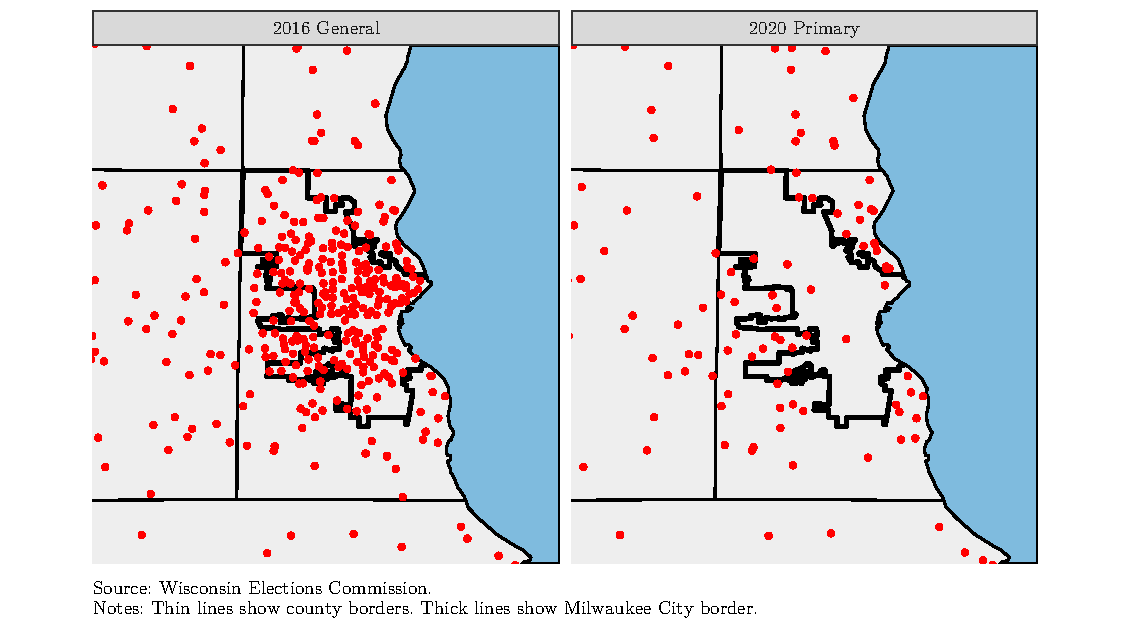
\includegraphics{mke_turnout-revised_files/figure-latex/map-1.pdf}
\caption{\label{fig:map}\label{fig:map}Polling Places in 2016 and 2020 Elections}
\end{figure}

Unfortunately, low-level data on the prevalence of COVID-19 on or before election day is unavailable. Shortly after the election the state began publishing counts at the census tract level, but these figures are not available for the period in which they were most relevant --- that is, before voters headed to the polls.

The April primary ballot included Democratic and Republican presidential primaries, a race for a seat on the state supreme court, seats on the state court of appeals and the state courts, and a statewide referendum. While Milwaukee County and the surrounding counties are in different Appeals Court districts, both judicial districts had race on the ballot, though the race in Milwaukee County was uncontested. At circuit court level, only Ozaukee County did not have a judicial race in the election. There is, in short, little cause for concern of unique campaign effects biasing our results. The only contextual differences between Milwaukee City and its suburbs are therefore the polling place consolidation and disparate prevalence of COVID-19.

To isolate the effect of polling place consolidation from COVID-19, we leverage electoral jurisdiction boundaries as an assignment to treatment mechanism (Kaplan and Yuan \protect\hyperlink{ref-Kaplan2020}{2020}; Cantoni \protect\hyperlink{ref-Cantoni2020}{2020}). Our primary design is a regression discontinuity in space that exploits the municipal boundary line to compare turnout for voters on either side of the ``cutpoint'' boundary (Keele, Titiunik, and Zubizarreta \protect\hyperlink{ref-Keele2015}{2015}). Research from New Orleans indicates that COVID-19 is clustered at the neighborhood level (van Holm, Wyczalkowski, and Dantzler \protect\hyperlink{ref-vanHolm2020}{2020}). Because of how close these voters lived to one another, it is likely they went about their daily lives in the same local milieu. Social geography has an effect on local politics and participation in elections (Enos \protect\hyperlink{ref-Enos2017}{2017}; Cho, Gimpel, and Dyck \protect\hyperlink{ref-Cho2006}{2006}; Gimpel, Dyck, and Shaw \protect\hyperlink{ref-Gimpel2004}{2004}). We therefore assume that, although they lived in different municipalities, the people proximate to each other but on either side of the municipal boundary were similarly exposed to COVID-19. Put differently, we \emph{directly} control for a host of covariates from the voter file, and we \emph{indirectly} control for COVID-19 by selecting pairs of treated and control voters who live in very close proximity to one another.

The regression discontinuity framework, however, assumes that individuals cannot ``select'' around the cutpoint; that within a narrow window individuals on either side of the cutpoint are identical. This is probably too strong of an assumption: voters likely select around the administrative boundary, a problem exacerbated by Milwaukee's extreme segregation. Keele, Titiunik, and Zubizarreta (\protect\hyperlink{ref-Keele2015}{2015}) suggests that, when selection around the cutpoint is a potential problem in a spatial regression discontinuity framework, implementing a matching algorithm can alleviate this problem: ``When there appears to be strong self-selection around the border of interest, one alternative is to combine designs and to assume that, after conditioning on covariates, treatment assignment is as-if randomized for those who live near the city limit'' (page 228). They combine regression discontinuity and matching methodologies, exploiting the Milwaukee City municipal boundary to investigate whether ballot initiatives increase turnout.

We adopt this approach by genetically matching each registered voter in Milwaukee City to two voters who live outside the city but in Milwaukee, Waukesha, Washington, or Ozaukee County, which each share a border with Milwaukee City.\footnote{There are 143 observations in the L2 data that are problematic. According to latitude and longitude coordinates these observations are within the boundary of Milwaukee City but are coded as outside the city. We omit these observations.} Genetic matching involves using an algorithm that ``automatically finds the set of matches that minimizes the discrepancy between the distribution of potential confounders in the treated and control groups'' (Sekhon \protect\hyperlink{ref-Sekhon2009}{2009}, 499). The villages of Whitefish Bay and Bayside sent mail ballot applications to all registered voters, potentially driving up their turnout relative to Milwaukee City (Gilbert \protect\hyperlink{ref-Gilbert2020}{2020}). We thus exclude these villages as potential controls.

Although these counties include some urban areas, we refer to the controls as suburban voters for convenience. To be sure, the vast majority of our eventual control voters live very close to the Milwaukee border --- and are thus in fact suburbanites in the traditional sense. Treated and control voters are matched exactly on turnout in the 2016 and 2018 primary elections, and on their partisan affiliation. Voters are also matched on their gender, their household income, whether they have a college education, and their race or ethnicity. Voters are also matched on their latitude and longitude to ensure physical proximity to one another.

Although this differs from a regression discontinuity in which there is a band around a cutpoint, the logic is the same. As the maximum allowed distance between treated and control voters approaches zero, we are in fact reducing the band around the cutpoint represented by the municipal border. For instance, when the maximum distance allowed between a treated voter and her match is 0.5 miles, each voter will live (on average) within 0.25 miles of the border. It is important to note that this is more conservative than matching treated and control voters within a buffer around the border --- not only must pairs both live within a buffer, they must also live near one another within that buffer.

By beginning with a strict geographic restriction, we isolate the causal effect of polling place consolidation on turnout. To estimate the net effect of polling place consolidation \emph{and} COVID-19, we then expand the maximum distance allowed between treated and control voters. While we cannot directly observe the effect of COVID-19, we can observe whether the overall treatment effect grows larger as we introduce more distance between the pairs. Because we have controlled for other relevant covariates, the only additional difference between treated and control voters will be their COVID-19 exposure.

Our results are likely to be somewhat conservative. Some municipalities outside of Milwaukee City reduced their number of polling places (see Figure \ref{fig:map}). This means some of our control voters received a very weak treatment --- therefore collapsing the difference between the treated and control voters and pushing our estimated treatment effect toward zero.

\hypertarget{results}{%
\subsubsection*{Results}\label{results}}
\addcontentsline{toc}{subsubsection}{Results}

We begin by presenting the results of the matching model, where each treated voter is matched with two control voters.\footnote{Due to computing constraints, we use a 1\% sample of voters (stratified by treatment status) \emph{to generate weights used in the actual matching model} though the whole pool is eventually used for the matching procedure itself.} Table \ref{tab:match} demonstrates that the matching procedure was largely successful: we achieve substantial improvement along all characteristics. Milwaukee City is far less white than the suburbs; has far lower incomes and education levels; and saw much lower turnout in recent primary elections. We do not include latitudes and longitudes in the balance table but the average distance between a treated voter and her controls is 2.3 miles. Matching is done with replacement, and ties are broken randomly.

\begin{singlespace}
\begin{table}[H]

\caption{\label{tab:balance-tab-chunk}\label{tab:match} Balance Table}
\centering
\resizebox{\linewidth}{!}{
\begin{tabular}[t]{lllllrrrr}
\toprule
\multicolumn{1}{c}{ } & \multicolumn{2}{c}{Means: Unmatched Data} & \multicolumn{2}{c}{Means: Matched Data} & \multicolumn{4}{c}{Percent Improvement} \\
\cmidrule(l{3pt}r{3pt}){2-3} \cmidrule(l{3pt}r{3pt}){4-5} \cmidrule(l{3pt}r{3pt}){6-9}
 & Treated & Control & Treated & Control & Mean Diff & eQQ Med & eQQ Mean & eQQ Max\\
\midrule
\% Voted in 2016 Primary & 26.8\% & 51.6\% & 26.8\% & 26.8\% & 100.00 & 100.00 & 100.00 & 100.00\\
\% Voted in 2018 Primary & 15.2\% & 27.9\% & 15.2\% & 15.2\% & 100.00 & 100.00 & 100.00 & 100.00\\
\% Male & 42.6\% & 45.5\% & 42.6\% & 42.6\% & 100.00 & 100.00 & 100.00 & 100.00\\
\% Democrats & 65.5\% & 20.7\% & 65.5\% & 65.5\% & 99.99 & 99.99 & 99.99 & 99.99\\
\% Republican & 8.6\% & 58.4\% & 8.6\% & 8.6\% & 99.99 & 99.99 & 99.99 & 99.99\\
Income & \$59,317 & \$99,255 & \$59,317 & \$59,334 & 99.96 & 99.96 & 99.91 & 99.83\\
\% with Collegiate Education & 12.7\% & 33.3\% & 12.7\% & 12.7\% & 100.00 & 100.00 & 100.00 & 100.00\\
\% White & 46.3\% & 76.0\% & 46.3\% & 46.3\% & 100.00 & 100.00 & 100.00 & 100.00\\
\% Black & 30.8\% & 0.9\% & 30.8\% & 30.8\% & 100.00 & 100.00 & 100.00 & 100.00\\
\% Latino & 8.8\% & 3.4\% & 8.8\% & 8.8\% & 100.00 & 100.00 & 100.00 & 100.00\\
\% Asian & 1.9\% & 1.7\% & 1.9\% & 1.9\% & 100.00 & 100.00 & 100.00 & 100.00\\
\bottomrule
\end{tabular}}
\end{table}
\end{singlespace}

Table \ref{tab:reg-table} presents the results of ordinary least squares regressions testing the treatment effect. In Table \ref{tab:reg-table} we require treated and control voters to live within 0.5 miles of one another.\footnote{A treated voter might live within the cutoff distance from one of her controls but not the other. The regression weights are updated for each regression to reflect this possibility.} For this reason, the number of observations in Table \ref{tab:reg-table} is relatively low: most Milwaukee voters do not live within 0.5 miles of the municipal border and a suburban control, and are thus excluded. In fact, just 13 percent of registered voters in Milwaukee City (and their matches) are included in this specification. The dependent variable takes the value 1 if a voter cast a ballot in the April primary, and 0 if she did not. We also test whether the treatment effect was different for Black voters than for other voters which Cantoni (\protect\hyperlink{ref-Cantoni2020}{2020}) indicates is possible. Models 1 and 3 include just the treatment variable (and, in Model 3, the interaction term) while Models 2 and 4 add in the variables on which the matching was performed (but without latitude and longitude).

\textbf{Of course, some important characteristics are unavailable at the individual-level and are thus not included in the matching procedure. We expect, however, that these will vary with the characteristics that are included. Car-ownership provides a helpful post-hoc test of the this assumption. Although car ownership is not included in the model, the average treated voter in Table \ref{tab:reg-table} lives in a census tract where 90.61 percent of households own cars; their controls live in neighborhoods where that figure is 90.64 percent. We thus have good reason to believe that the matching procedure reduces differences between treated and control voters even for characteristics not directly included.}

Although COVID-19 data is not available prior to the election, the Department of Health Services began releasing this data at the census tract level shortly after the election. We use cumulative positivity rates from April 21 --- two weeks after the election --- to proxy potential COVID-19 rates as of the election as a robustness check in Model 5. Insofar as these are correlated with COVID prevalence on election day, they may be probative to the direct effect of COVID-19 on turnout.\footnote{Positive test rates are calculated as positive counts divided by the sum of positive and negative counts. The Department of Health Services replaces counts of less than 5 COVID-19 cases with ``-999;'' we re-code these as the mean value ``2.'' See: \url{https://data.dhsgis.wi.gov/datasets/covid-19-historical-data-table}.} However, because the COVID data is not available as of the primary election, Model 5 is not intended to provide definitive proof of the relationship between virus prevalence and turnout. In each model, robust standard errors are clustered at the level of the match (Abadie and Spiess \protect\hyperlink{ref-Abadie2019}{2019}).

\begin{singlespace}

\input{"../temp/reg.tex"}
\end{singlespace}

Models 1 and 2 indicate that turnout was depressed by roughly 8.7 percentage points in the April primary in Milwaukee City relative to suburban voters. Models 3 and 4 indicate that this decrease was especially pronounced among Black voters, who saw turnout nearly \textbf{10.4} percentage points below that of their suburban matches. Model 5 shows no significant turnout effect where a higher share of cumulative COVID-19 tests were positive two weeks after the election. The large treatment effect supports Hypothesis A.

We are also interested in whether the size of the treatment effect grows as we include pairs who live further away from one another. Figure \ref{fig:coef-plot} re-estimates of Model 3 from Table \ref{tab:reg-table} using different maximum distances between pairs. As the maximum distance between treated and control voters grows, the number of observations also grows to include all registered voters in Milwaukee City and their matches.

\begin{figure}
\centering
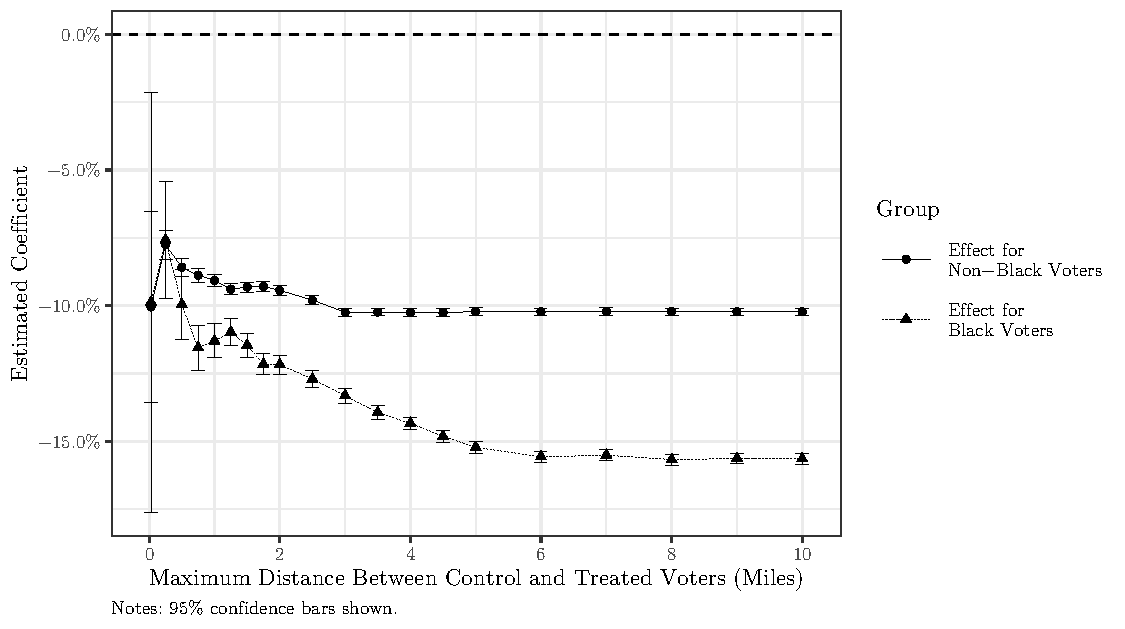
\includegraphics{mke_turnout-revised_files/figure-latex/plot-1.pdf}
\caption{\label{fig:plot}\label{fig:coef-plot}Estimated Depressive Effect of Living in Milwaukee, 2020 Primary}
\end{figure}

\textbf{As the maximum distance between treated and control voters increases, the overall depressive effect and interaction effect grow in magnitude. It is important to note that this is not due to different underlying propensities to vote: the matching procedure requires that the participation (or lack thereof) of treated voters in the 2016 and 2018 primaries is exactly mirrored by their controls. The difference in overall treatment effect between the half-mile and most lenient models is roughly 1.3 percentage points (the interaction effect grows by 4.7 percentage points). Thus COVID-19 likely reduced turnout relative to the suburbs (through mechanisms other than polling place consolidation) by 1.3 percentage points for non-Black voters, and as much as 6.0 percentage points for Black voters. Given the extreme racial disparities of COVID-19 in Wisconsin (Hayda \protect\hyperlink{ref-Hayda2020}{2020}) it is unsurprising that these ``direct effects'' are so much greater for Black voters. This provides evidence to support Hypothesis B.}

\hypertarget{discussion}{%
\subsubsection*{Discussion}\label{discussion}}
\addcontentsline{toc}{subsubsection}{Discussion}

On the one hand, polling place closures have long been understood to reduce turnout among voters. On the other hand, when jurisdictions have switched to primarily vote by mail systems, turnout has hardly changed. In the face of COVID-19, it was unclear how closed polling places would affect turnout. The enormous surge in absentee ballots indicated that the negative turnout effects might not have been large, but reporting of extensive lines for in-person voting on election day in Milwaukee (Viebeck et al. \protect\hyperlink{ref-Viebeck2020}{2020}) led us to expect that there were measurable negative turnout effects.

This note makes clear that polling place closures reduced turnout in the April primary in Milwaukee in the context of COVID-19, despite unprecedented demand for absentee ballots. The \textbf{8.7} percentage point decrease we observe is quite large; this effect amounts to about a third of the 26.1 percent turnout among control voters. \textbf{This demobilizing effect in Wisconsin is not nonlinear as the distance threshold increases, as we would expect from earlier studies; rather the effect nearly constant beyond anything but the closest distances.} The case of Milwaukee also sheds some light on the direct effect of COVID-19 on turnout. We know that COVID-19 was more widespread in Milwaukee City at the time of the election. Expanding the distance between treated and control voters led to larger treatment effects. Because the only thing varying in these specifications was space --- and, therefore, COVID-19 exposure --- this provides some evidence that COVID-19 directly reduced turnout even though our most restrictive regression found no significant effect.

These data have two boundary conditions it is important to bear in mind. First, the onset of the pandemic and the timing of the April primary did not allow time for a robust public messaging campaign about mail voting options and it may be the case that the August and November elections, held after the initial phase of the pandemic, saw smaller effects due to less severe polling place consolidation. The City of Milwaukee may well have learned from their April experience: in the August partisan primary, there were 168 polling places open in the city.\footnote{See \url{https://elections.wi.gov/node/6527}.} Second, it may be the case that the larger depressive effect for Black rather than for non-Black voters that we observe is a product of the relatively high segregation rate in Milwaukee compared to other American cities. Why polling place consolidation disproportionately depressed turnout among Black voters is unclear and should be the focus of future research based in other localities. This finding, nonetheless, raises concerns about racial representation when jurisdictions are forced by a natural emergency to consolidate polling places.

This note answers just one question related to the effect of COVID-19: given the pandemic, how do polling place closures affect turnout? Future research must consider the overall turnout and representational impacts of COVID-19 on this year's contests. It is worth noting that recently published research found that the April primary was not linked to any surge in COVID-19 in Wisconsin (Leung et al. \protect\hyperlink{ref-Leung2020}{2020}), which should allay concerns that polling places can only be kept open at the expense of public health. The primary elections in Milwaukee, Wisconsin, make one thing clear: even as many voters transition to vote-by-mail in the face of a pandemic, polling place consolidation can still have disenfranchising effects --- particularly for Black voters.

\newpage

\hypertarget{references}{%
\subsubsection*{References}\label{references}}
\addcontentsline{toc}{subsubsection}{References}

\hypertarget{refs}{}
\begin{cslreferences}
\leavevmode\hypertarget{ref-Abadie2019}{}%
Abadie, Alberto, and Jann Spiess. 2019. ``Robust Post-Matching Inference.'' \emph{Working Paper.}

\leavevmode\hypertarget{ref-Bergman2015}{}%
Bergman, Elizabeth. 2015. ``Voting Only by Mail Can Decrease Turnout. Or Increase It. Wait, What?'' \emph{Washington Post}, December 21, 2015. \url{https://www.washingtonpost.com/news/monkey-cage/wp/2015/12/21/voting-only-by-mail-can-decrease-or-increase-turnout-wait-what/}.

\leavevmode\hypertarget{ref-Bergman2011}{}%
Bergman, Elizabeth, and Philip Yates. 2011. ``Changing Election Methods: How Does Mandated Vote-by-Mail Affect Individual Registrants?'' \emph{Election Law Journal} 10 (2): 115--27.

\leavevmode\hypertarget{ref-Brady2011}{}%
Brady, Henry E., and John E. Mcnulty. 2011. ``Turning Out to Vote: The Costs of Finding and Getting to the Polling Place.'' \emph{American Political Science Review} 105 (1): 115--34. \url{https://doi.org/10.1017/S0003055410000596}.

\leavevmode\hypertarget{ref-Cantoni2020}{}%
Cantoni, Enrico. 2020. ``A Precinct Too Far: Turnout and Voting Costs.'' \emph{American Economic Journal: Applied Economics} 12 (1): 61--85.

\leavevmode\hypertarget{ref-Cho2006}{}%
Cho, Wendy, James Gimpel, and Joshua Dyck. 2006. ``Residential Concentration, Political Socialization, and Voter Turnout.'' \emph{Journal of Politics} 68 (1): 156--67. \url{https://doi.org/10.1111/j.1468-2508.2006.00377.x}.

\leavevmode\hypertarget{ref-Cortina2019}{}%
Cortina, Jeronimo, and Brandon Rottinghaus. 2019. ``Vote Centers and Turnout by Election Type in Texas.'' \emph{Research and Politics} 6 (3): 1--7. \url{https://doi.org/10.1177\%2F2053168019864224}.

\leavevmode\hypertarget{ref-Dyck2005}{}%
Dyck, Joshua, and James Gimpel. 2005. ``Distance, Turnout, and the Convenience of Voting.'' \emph{Social Science Quarterly} 86 (3): 531--48.

\leavevmode\hypertarget{ref-Elul2017}{}%
Elul, Gabrielle, Sean Freeder, and Jacob Grumbach. 2017. ``The Effect of Mandatory Mail Ballot Elections in California.'' \emph{Election Law Journal} 16 (3): 397--415.

\leavevmode\hypertarget{ref-Enos2017}{}%
Enos, Ryan. 2017. \emph{The Space Between Us: Social Geography and Politics}. Cambridge: Cambridge University Press.

\leavevmode\hypertarget{ref-Frey2018}{}%
Frey, William H. 2018. ``Black-White Segregation Edges Downward Since 2000, Census Shows.'' Brookings. \url{https://www.brookings.edu/blog/the-avenue/2018/12/17/black-white-segregation-edges-downward-since-2000-census-shows/}.

\leavevmode\hypertarget{ref-Gerber2013}{}%
Gerber, Alan, Gregory Huber, and Seth Hill. 2013. ``Identifying the Effect of All-Mail Elections on Turnout: Staggered Reform in the Evergreen State.'' \emph{Political Science Research and Methods} 1 (1): 91--116.

\leavevmode\hypertarget{ref-Gerken2007}{}%
Gerken, Heather. 2007. \emph{The Democracy Index: Why Our Election System Is Failing and How to Fix It}. Princeton: Princeton University Press.

\leavevmode\hypertarget{ref-Gilbert2020}{}%
Gilbert, Craig. 2020. ``How Two Communities on Milwaukee's North Shore Achieved Sky-High Levels of Absentee Voting Despite Coronavirus.'' \emph{Milwaukee Journal Sentinel}, April 10, 2020. \url{https://www.jsonline.com/story/news/politics/elections/2020/04/10/wisconsin-absentee-ballot-forms-sent-whitefish-bay-bayside-voters/5129125002/}.

\leavevmode\hypertarget{ref-Gimpel2004}{}%
Gimpel, James, Joshua Dyck, and Daron Shaw. 2004. ``Registrants, Voters, and Turnout Variability Across Neighborhoods.'' \emph{Political Behavior} 26 (4): 375.

\leavevmode\hypertarget{ref-Gimpel2003}{}%
Gimpel, James, and Jason Schuknecht. 2003. ``Political Participation and the Accessibility of the Ballot Box.'' \emph{Political Geography} 22: 471--88.

\leavevmode\hypertarget{ref-Gronke2012}{}%
Gronke, Paul, and Peter Miller. 2012. ``Voting by Mail and Turnout in Oregon: Revisiting Southwell and Burchett.'' \emph{American Politics Research} 40 (6): 976--97. \url{https://doi.org/10.1177/1532673X12457809}.

\leavevmode\hypertarget{ref-Haspel2005}{}%
Haspel, Moshe, and H. Gibbs Knotts. 2005. ``Location, Location, Location: Precinct Placement and the Costs of Voting.'' \emph{Journal of Politics} 67 (2): 560--73.

\leavevmode\hypertarget{ref-Hayda2020}{}%
Hayda, Julian. 2020. ``Wisconsin's COVID-19 Death Disparity Is 3rd Worst in America. Is Segregation to Blame?'' \emph{WUWM}, May 29, 2020. \url{https://www.wuwm.com/post/wisconsins-covid-19-death-disparity-3rd-worst-america-segregation-blame}.

\leavevmode\hypertarget{ref-Henrickson2019}{}%
Henrickson, Kevin E., and Erica H. Johnson. 2019. ``Increasing Voter Participation by Altering the Costs and Stakes of Voting*.'' \emph{Social Science Quarterly} 100 (3): 869--84. \url{https://doi.org/10.1111/ssqu.12583}.

\leavevmode\hypertarget{ref-Hobbs2014}{}%
Hobbs, William R., Nicholas A. Christakis, and James H. Fowler. 2014. ``Widowhood Effects in Voter Participation.'' \emph{American Journal of Political Science} 58 (1): 1--16. \url{https://doi.org/10.1111/ajps.12040}.

\leavevmode\hypertarget{ref-vanHolm2020}{}%
Holm, Eric Joseph van, Christopher Wyczalkowski, and Prentiss Dantzler. 2020. ``Neighborhood Conditions and the Initial Outbreak of COVID-19: The Case of Louisiana.'' SSRN Scholarly Paper ID 3625990. Rochester, NY: Social Science Research Network. \url{https://doi.org/10.2139/ssrn.3625990}.

\leavevmode\hypertarget{ref-Huefner2007}{}%
Huefner, Steven, Daniel Tokaji, Edward Foley, and Nathan Cemenska. 2007. \emph{From Registration to Recounts: The Election Ecosystems of Five Midwestern States}. Columbus: The Ohio State University Michael E. Moritz College of Law.

\leavevmode\hypertarget{ref-Kaplan2020}{}%
Kaplan, Ethan, and Haishan Yuan. 2020. ``Early Voting Laws, Voter Turnout, and Partisan Vote Composition: Evidence from Ohio.'' \emph{American Economic Journal: Applied Economics} 12 (1): 32--60.

\leavevmode\hypertarget{ref-Keele2015}{}%
Keele, Luke, Rocío Titiunik, and José R. Zubizarreta. 2015. ``Enhancing a Geographic Regression Discontinuity Design Through Matching to Estimate the Effect of Ballot Initiatives on Voter Turnout.'' \emph{Journal of the Royal Statistical Society: Series A (Statistics in Society)} 178 (1): 223--39. \url{https://doi.org/10.1111/rssa.12056}.

\leavevmode\hypertarget{ref-Kimball2013}{}%
Kimball, David, and Brady Baybeck. 2013. ``Are All Jurisdictions Equal? Size Disparity in Election Administration.'' \emph{Election Law Journal} 12 (2): 130--45. \url{https://doi.org/10.1089/elj.2012.0174}.

\leavevmode\hypertarget{ref-Kousser2007}{}%
Kousser, Thad, and Megan Mullin. 2007. ``Does Voting by Mail Increase Participation? Using Matching to Analyze a Natural Experiment.'' \emph{Political Analysis} 15 (4): 428--45. \url{http://www.jstor.org/stable/25791905}.

\leavevmode\hypertarget{ref-Kropf2012}{}%
Kropf, Martha E., and David C. Kimball. 2012. \emph{Helping America Vote: The Limits of Election Reform}. New York ; London: Routledge.

\leavevmode\hypertarget{ref-Leung2020}{}%
Leung, Kathy, Joseph T. Wu, Kuang Xu, and Lawrence M. Wein. 2020. ``No Detectable Surge in SARS-CoV-2 Transmission Attributable to the April 7, 2020 Wisconsin Election.'' \emph{American Journal of Public Health} 110 (8): 1169--70. \url{https://doi.org/10.2105/AJPH.2020.305770}.

\leavevmode\hypertarget{ref-Marley2020}{}%
Marley, Patrick, and Molly Beck. 2020. ``Lack of Poll Workers Across Wisconsin, Flood of Absentee Ballots Spark Fears Votes Will Go Uncounted.'' \emph{Milwaukee Journal Sentinel}, March 31, 2020. \url{https://www.jsonline.com/story/news/politics/elections/2020/03/31/coronavirus-wisconsin-tony-evers-asks-state-workers-staff-polls/5093547002/}.

\leavevmode\hypertarget{ref-McNulty2009}{}%
McNulty, John, Conor Dowling, and Margaret Ariotti. 2009. ``Driving Saints to Sin: How Increasing the Difficulty of Voting Dissuades Even the Most Motivated Voters.'' \emph{Political Analysis} 17 (4): 435--55.

\leavevmode\hypertarget{ref-Mickle2020}{}%
Mickle, Jordan. 2020. ``Five Voting Centers, Five Absentee Ballot Drop-Off Locations Open in Milwaukee for Tuesday's Primary.'' \emph{TMJ4 Milwaukee: Local News}, April 6, 2020. \url{https://www.tmj4.com/news/local-news/these-are-the-five-in-person-voting-centers-in-milwaukee-open-for-wisconsins-spring-primary-tuesday}.

\leavevmode\hypertarget{ref-Pacheco2015}{}%
Pacheco, Julianna, and Jason Fletcher. 2015. ``Incorporating Health into Studies of Political Behavior: Evidence for Turnout and Partisanship.'' \emph{Political Research Quarterly} 68 (1): 104--16. \url{https://doi.org/10.1177/1065912914563548}.

\leavevmode\hypertarget{ref-Rosenstone1982}{}%
Rosenstone, Steven J. 1982. ``Economic Adversity and Voter Turnout.'' \emph{American Journal of Political Science} 26 (1): 25--46. \url{https://doi.org/10.2307/2110837}.

\leavevmode\hypertarget{ref-Sekhon2009}{}%
Sekhon, Jasjeet. 2009. ``Opiates for the Matches: Matching Methods for Causal Inference.'' \emph{Annual Review of Political Science} 12: 487--508.

\leavevmode\hypertarget{ref-Stein2008}{}%
Stein, Robert M., and Greg Vonnahme. 2008. ``Engaging the Unengaged Voter: Vote Centers and Voter Turnout.'' \emph{The Journal of Politics} 70 (2): 487--97. \url{https://doi.org/10.1017/S0022381608080456}.

\leavevmode\hypertarget{ref-Stein2012}{}%
Stein, Robert, and Greg Vonnahme. 2012. ``Effect of Election Day Vote Centers on Voter Participation.'' \emph{Election Law Journal} 11 (3): 291--301. \url{https://doi.org/10.1089/elj.2011.0101}.

\leavevmode\hypertarget{ref-Stewart2010}{}%
Stewart, Charles. 2010. ``Losing Votes by Mail.'' \emph{New York University Journal of Legislation and Public Policy} 13: 573--602.

\leavevmode\hypertarget{ref-Viebeck2020}{}%
Viebeck, Elise, Amy Gardner, Dan Simmons, and Jan M. Larson. 2020. ``Long Lines, Anger and Fear of Infection: Wisconsin Proceeds with Elections Under Court Order.'' \emph{Washington Post}, April 7, 2020. \url{https://www.washingtonpost.com/politics/long-lines-form-in-milwaukee-as-wisconsin-proceeds-with-elections-under-court-order/2020/04/07/93727b34-78c7-11ea-b6ff-597f170df8f8_story.html}.

\leavevmode\hypertarget{ref-Wise2020}{}%
Wise, David. 2020. ``Evers Calls for All Voters to Be Mailed Absentee Ballots \textbar{} WisPolitics.Com.'' \emph{WisPolitics}, March 27, 2020. \url{https://www.wispolitics.com/2020/evers-calls-for-all-voters-to-be-mailed-absentee-ballots/}.
\end{cslreferences}

\end{document}
